\documentclass[11pt]{article}

% --- Page & typography (tight) ---
\usepackage[a4paper,margin=0.9in]{geometry}
\usepackage{amsmath,amssymb,mathtools}
\usepackage{tikz}
\usetikzlibrary{positioning, shapes, arrows.meta}
\usepackage{graphicx}
\usepackage{microtype}
\usepackage{titlesec}
\usepackage{enumitem}
\usepackage{hyperref}
\hypersetup{colorlinks=true, linkcolor=black, urlcolor=black, citecolor=black}
\begin{document}

\begin{figure}[h!]
\centering
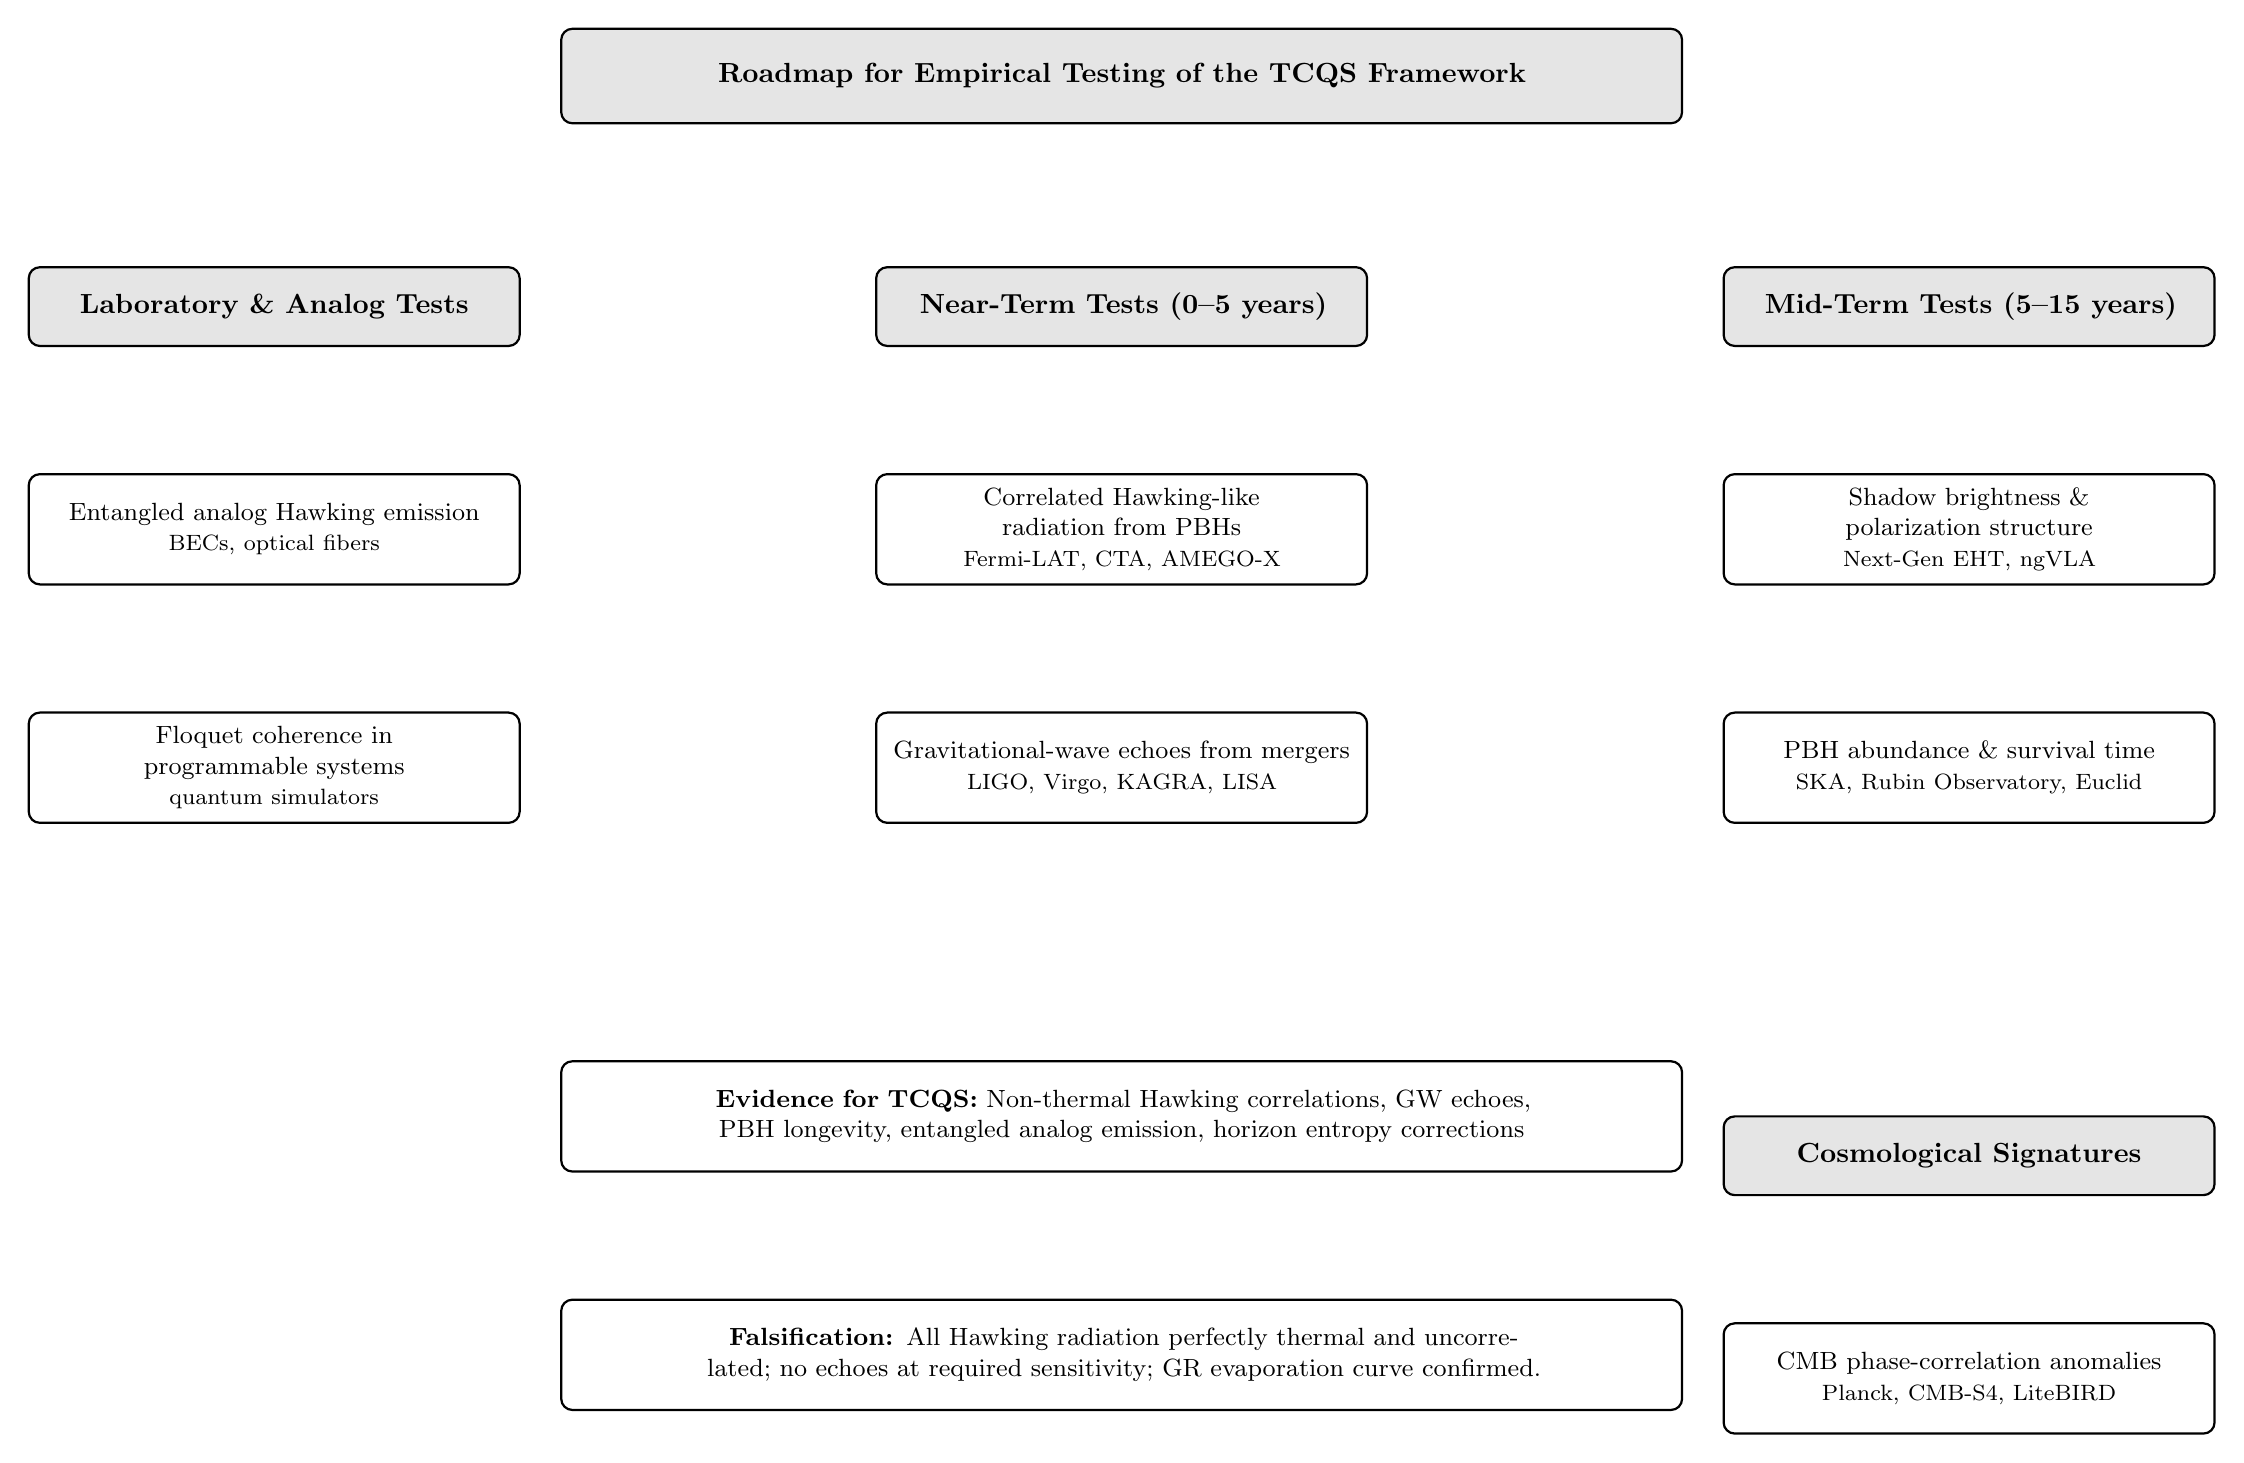
\begin{tikzpicture}[
    node distance=1.6cm,
    box/.style={
        rectangle, rounded corners,
        draw=black, thick,
        align=center,
        text width=6cm,
        minimum height=1.4cm,
        font=\small
    },
    title/.style={
        rectangle, rounded corners,
        draw=black, thick,
        fill=black!10,
        font=\bfseries,
        text width=6cm,
        minimum height=1cm,
        align=center
    }
]

% Title
\node[title,text width=14cm,minimum height=1.2cm] (title)
{Roadmap for Empirical Testing of the TCQS Framework};

% Near-term
\node[title,below=of title,yshift=-0.2cm] (near)
{Near-Term Tests (0–5 years)};
\node[box,below=of near] (nearA)
{Correlated Hawking-like radiation from PBHs \\
{\footnotesize Fermi-LAT, CTA, AMEGO-X}};
\node[box,below=of nearA] (nearB)
{Gravitational-wave echoes from mergers \\
{\footnotesize LIGO, Virgo, KAGRA, LISA}};

% Mid-term
\node[title,right=4.5cm of near] (mid)
{Mid-Term Tests (5–15 years)};
\node[box,below=of mid] (midA)
{Shadow brightness \& polarization structure \\
{\footnotesize Next-Gen EHT, ngVLA}};
\node[box,below=of midA] (midB)
{PBH abundance \& survival time \\
{\footnotesize SKA, Rubin Observatory, Euclid}};

% Laboratory
\node[title,left=4.5cm of near] (lab)
{Laboratory \& Analog Tests};
\node[box,below=of lab] (labA)
{Entangled analog Hawking emission \\
{\footnotesize BECs, optical fibers}};
\node[box,below=of labA] (labB)
{Floquet coherence in programmable systems \\
{\footnotesize quantum simulators}};

% Cosmology
\node[title,below=3.7cm of midB] (cosmo)
{Cosmological Signatures};
\node[box,below=of cosmo] (cosmoA)
{CMB phase-correlation anomalies \\
{\footnotesize Planck, CMB-S4, LiteBIRD}};

% Success & Failure
\node[box,below=3cm of nearB,text width=14cm] (success)
{\textbf{Evidence for TCQS:}
Non-thermal Hawking correlations, GW echoes, PBH longevity,
entangled analog emission, horizon entropy corrections};

\node[box,below=of success,text width=14cm] (failure)
{\textbf{Falsification:}
All Hawking radiation perfectly thermal and uncorrelated;
no echoes at required sensitivity; GR evaporation curve confirmed.};

\end{tikzpicture}
\caption{A structured, instrument-driven roadmap for experimentally testing the TCQS framework.}
\end{figure}
\end{document}